% ATC-MAS -- Task 1 (Design activity) report
% IEEE template (IEEEtran, conference style), one column.
% Build:  cd docs/task1 && latexmk -pdf main.tex
% Each section lives in sections/ with NO preamble; one owner per file (see roadmap section 3).

\documentclass[conference,onecolumn,a4paper,11pt]{IEEEtran}

% ===== PACKAGES =====
\usepackage[T1]{fontenc}
\usepackage[utf8]{inputenc}
\usepackage{cite}
\usepackage{amsmath,amssymb}
\usepackage{booktabs}
\usepackage{array}
\usepackage{tabularx}
\let\labelindent\relax              % IEEEtran and enumitem both define \labelindent
\usepackage{enumitem}
\usepackage{graphicx}
\usepackage{float}
\usepackage{xcolor}
\usepackage{pifont}
\usepackage{tikz}
\usetikzlibrary{arrows.meta,positioning,shapes.geometric}
\usepackage{tcolorbox}
\usepackage{url}

% Shared palette (same file as the slides, so colours cannot drift)
% Shared ATC-MAS palette for Task 1.
% \input by both the report (docs/task1/) and the slides (docs/task1/slides/)
% so the two documents cannot drift apart. Values match PR #3.
% Requires xcolor (loaded automatically by beamer).

\definecolor{atcnavy}{RGB}{20,45,80}        % #142D50
\definecolor{atcamber}{RGB}{220,150,30}     % #DC961E
\definecolor{atclightblue}{RGB}{190,215,240}
\definecolor{atcred}{RGB}{190,45,45}
\definecolor{atcgreen}{RGB}{40,130,75}
\definecolor{atcslate}{RGB}{90,100,115}

% Used by the slides (block titles and backgrounds)
\definecolor{atcblue}{RGB}{40,117,167}      % #2875A7
\definecolor{atclight}{RGB}{242,245,249}    % #F2F5F9


\usepackage[hidelinks]{hyperref}

% Boxed justification used in the agent section (from PR #3)
\newtcolorbox{successbox}[1][]{
    colback=green!5,
    colframe=green!50!black,
    title=#1,
    fonttitle=\bfseries
}

% Visible placeholder for text not written yet
\newcommand{\placeholder}[1]{\textcolor{atcred}{\textit{[#1]}}}

\begin{document}

% ===== TITLE =====
\title{Air Traffic Control Multi-Agent System\\
       \large Task 1: Design Activity}

% TODO(each member): check the spelling of your own name (same list as slide 1).
\author{\IEEEauthorblockN{Aram Abrahamyan, Fardin Ahmed, Soham Chakraborty,\\
                          Luis David Landicho Antonio, Bhavan Mullur Gopal, Vinay Narayanappa}
\IEEEauthorblockA{ATC-MAS Team 6\\
                  Multi-Agent Systems -- MAI, ETSE-URV\\
                  November 2026}}

\maketitle

\begin{abstract}
\placeholder{Abstract (Aram): 4--6 sentences summarising the problem, the five crews, the flow and the main design choices. Write it last.}
\end{abstract}

\begin{IEEEkeywords}
multi-agent systems, air traffic control, conflict detection and resolution, CrewAI, agent taxonomy
\end{IEEEkeywords}

% Owner: Aram
% No preamble here: only the section body. Packages and colours come from ../main.tex.
% Cite sources with keys from ../refs.bib (e.g. \cite{urvlect2}).
% Guidance: problem, why a MAS, scope and assumptions, report structure (roadmap task table, task 2).
\section{Introduction}\label{sec:intro}

\placeholder{To be written by Aram.}
                 % Aram
% Owner: Aram
% No preamble here: only the section body. Packages and colours come from ../main.tex.
% Cite sources with keys from ../refs.bib (e.g. \cite{urvlect2}).
% Guidance: inputs, crews table, flow figure (same TikZ as slide 3), routers A/B/C, design principle (roadmap 2.1-2.3).
\section{System Overview}\label{sec:overview}

\placeholder{To be written by Aram.}
              % Aram (figure shared with slide 3)
% Owner: ekagrahvinay-netizen
% Section body only; packages and colours are loaded by ../main.tex.
% Based on the five categories in the team's Lecture 2 environment slide.
\section{Environment Analysis}\label{sec:environment}

The Air Traffic Control Multi-Agent System (ATC-MAS) is designed for a
\emph{simulated, batch-processing} environment, not live air traffic control.
It reads a GraphML airspace network and JSON aircraft and flight-plan data,
validates them, and predicts aircraft trajectories to identify possible
separation conflicts. The model uses horizontal and vertical separation
thresholds of 5 nautical miles and 1000 feet, respectively \cite{icao4444}. We classify
its environment using the five properties discussed in Lecture 2
\cite{urvlect2,wooldridge2009}; an analogous, broader classification appears in~\cite{russell2020}.

\subsection{Environment Characteristics}

\paragraph{Accessible versus inaccessible}
Real ATC is \emph{inaccessible}: surveillance can be noisy or incomplete,
and pilot intentions cannot always be observed. Our \emph{modelled scenario}
is classified as \emph{accessible}, because the simulation receives the
scenario information required by its calculations. This does not imply
that every agent has access to all data; individual crews may receive only
the information needed to perform their roles.

\paragraph{Deterministic versus non-deterministic}
Real ATC is \emph{non-deterministic}: weather, aircraft behaviour and pilot
responses introduce uncertainty. The simulated trajectory and conflict
calculations are \emph{deterministic} for the same valid inputs and fixed
rules. Outputs proposed by language-model-based agents may still vary;
such proposals should not be confused with the deterministic safety checks.

\paragraph{Episodic versus non-episodic}
Real ATC is \emph{non-episodic}, since a clearance can affect later traffic
situations and decisions. Our simulation is \emph{episodic across runs}:
each submitted scenario is processed independently. It is
\emph{non-episodic within a run}, because conflict findings and subsequent
resolution decisions depend on earlier processing steps.

\paragraph{Static versus dynamic}
Real ATC is \emph{dynamic}, since aircraft keep moving and conditions
change while decisions are made. The simulated scenario is \emph{static}
with respect to external inputs during each batch run: no new live radar
or weather observations arrive. This does not mean the model ignores
motion; positions change along the trajectories being calculated.

\paragraph{Discrete versus continuous}
Real aircraft movement is predominantly \emph{continuous}: position,
time, altitude and speed vary continuously. Our simulation is
\emph{hybrid and discretised by design}: graph routes and a finite set of manoeuvres coexist with numerical trajectory
quantities. Candidate resolutions must still be assessed against the
model's numerical separation constraints.

\subsection{Implications for System Design}

These characteristics motivate a separation of deterministic verification
from agent coordination. Data Management validates the supplied files,
and Surveillance \& Conflict calculates potential separation violations.
Conflict-free scenarios proceed to Reporting; scenarios with conflicts
are routed to Tactical Resolution. The Safety Validation \& QA crew
independently checks suggested manoeuvres, rejecting unsafe alternatives
and allowing bounded retries before reporting the final status.

Because the environment is accessible, deterministic and static during
a run, the system can afford deliberative planning: as Lecture~2 notes,
planning with an explicit model of the world can reach optimal solutions
when the environment does not change while the plan is being
made~\cite{urvlect2}. At the same time, the environment is non-episodic
within a run: a manoeuvre that resolves one conflict can create another.
This is why every proposed manoeuvre is re-checked by the independent
Safety Validation \& QA crew before it is reported.

The resulting design supports deliberative coordination without treating
language-model output as a safety guarantee. This is an academic
simulation, not a real-world clearance system.

           % ekagrahvinay-netizen

\section{Agent Selection \& Multi-Crew Architecture}

\subsection{Architectural Addition: Safety Validation \& Quality Assurance Crew}

The proposed ATC-MAS architecture is organised into five specialised crews: Data Management, Surveillance \& Conflict, Tactical Resolution, Safety Validation \& Quality Assurance, and Reporting. The first four responsibilities originate from the main system workflow. We introduce exactly one additional crew, the Safety Validation \& Quality Assurance Crew, to provide an independent review of proposed flight-plan changes.

This additional crew addresses an important safety consideration in air traffic management: resolving one conflict does not necessarily guarantee that the resulting flight plans are safe. For example, changing Aircraft A's route to avoid Aircraft B could introduce a new conflict with Aircraft C. Therefore, proposed changes must be checked against the other aircraft in the scenario before a final clearance decision is made.

The separation of planning and validation also avoids having the same crew both propose and certify its own changes. An independent validation crew can assess the revised plans, identify secondary conflicts, and reject proposals that do not satisfy the defined safety constraints. This separation also makes the validation process independently assessable.

Weather information, where available, is treated as an optional input to the constraint-checking process rather than as a separate crew.

\begin{figure}[htbp]
\centering
\resizebox{\textwidth}{!}{%
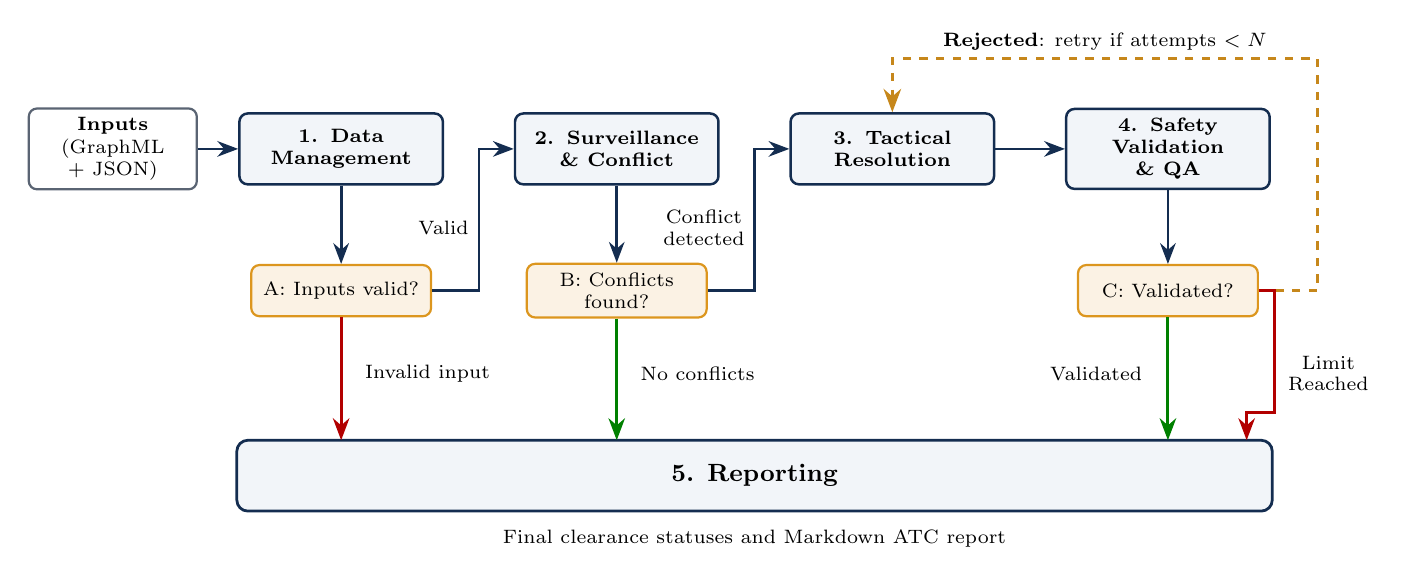
\begin{tikzpicture}[
    >=Stealth,
    crew/.style={
        draw=atcnavy,
        fill=atclight,
        rounded corners=3pt,
        line width=0.9pt,
        minimum width=2.55cm,
        minimum height=0.90cm,
        text width=2.35cm,
        align=center,
        font=\scriptsize\bfseries
    },
    decision/.style={
        draw=atcamber,
        fill=atcamber!12,
        rounded corners=3pt,
        line width=0.8pt,
        minimum width=2.25cm,
        minimum height=0.65cm,
        text width=2.05cm,
        align=center,
        font=\scriptsize
    },
    process/.style={
        ->,
        draw=atcnavy,
        line width=1pt
    },
    success/.style={
        ->,
        draw=green!50!black,
        line width=1.1pt
    },
    exception/.style={
        ->,
        draw=red!70!black,
        line width=1.1pt
    },
    retry/.style={
        ->,
        draw=atcamber!90!black,
        dashed,
        line width=1.2pt
    },
    lab/.style={
        font=\scriptsize,
        fill=white,
        inner sep=2pt
    }
]

% ==========================================
% ROW 1: PROCESSING CREWS
% ==========================================

\node[
    draw=atcslate,
    fill=white,
    rounded corners=3pt,
    line width=0.8pt,
    minimum height=0.90cm,
    text width=1.9cm,
    align=center,
    font=\scriptsize
] (inputs) at (-2.9,0)
    {\textbf{Inputs}\\(GraphML + JSON)};

\node[crew] (dm) at (0,0)
    {1. Data\\Management};

\node[crew] (sc) at (3.5,0)
    {2. Surveillance\\\& Conflict};

\node[crew] (tr) at (7.0,0)
    {3. Tactical\\Resolution};

\node[crew] (sv) at (10.5,0)
    {4. Safety\\Validation \& QA};

% ==========================================
% ROW 2: DECISIONS
% ==========================================

\node[decision] (a) at (0,-1.8)
    {A: Inputs valid?};

\node[decision] (b) at (3.5,-1.8)
    {\shortstack{B: Conflicts\\found?}};

\node[decision] (c) at (10.5,-1.8)
    {C: Validated?};

% ==========================================
% ROW 3: SHARED REPORTING DESTINATION
% ==========================================

\node[
    draw=atcnavy,
    fill=atclight,
    rounded corners=4pt,
    line width=1pt,
    minimum width=13.15cm,
    minimum height=0.90cm,
    align=center,
    font=\small\bfseries
] (report) at (5.25,-4.15)
    {5. Reporting};

% Explicit ports on the reporting bar
\coordinate (rA) at (0,-3.70);
\coordinate (rB) at (3.5,-3.70);
\coordinate (rC) at (10.5,-3.70);
\coordinate (rEnd) at (11.5,-3.70);

% ==========================================
% CREW -> DECISION
% ==========================================

\draw[process] (inputs.east) -- (dm.west);
\draw[process] (dm.south) -- (a.north);
\draw[process] (sc.south) -- (b.north);
\draw[process] (sv.south) -- (c.north);

% ==========================================
% A: VALID INPUT -> SURVEILLANCE
% ==========================================

\draw[process]
    (a.east) -- (1.75,-1.8)
    -- (1.75,0)
    -- (sc.west);

\node[lab] at (1.30,-1.0) {Valid};

% A: INVALID INPUT -> REPORTING
\draw[exception]
    (a.south) -- (rA);

\node[
    font=\scriptsize,
    anchor=west,
    fill=white
] at (0.18,-2.85)
    {Invalid input};

% ==========================================
% B: CONFLICT FOUND -> TACTICAL
% ==========================================

\draw[process]
    (b.east) -- (5.25,-1.8)
    -- (5.25,0)
    -- (tr.west);

\node[
    font=\scriptsize,
    anchor=east,
    align=center,
    fill=white,
    inner sep=2pt
] at (5.20,-1.0)
    {\shortstack{Conflict\\detected}};

\draw[success]
    (b.south) -- (rB);

\node[
    font=\scriptsize,
    anchor=west,
    fill=white
] at (3.68,-2.85)
    {No conflicts};

% ==========================================
% TACTICAL -> SAFETY VALIDATION
% ==========================================

\draw[process] (tr.east) -- (sv.west);

% ==========================================
% C: VALIDATED -> REPORTING
% ==========================================

\draw[success]
    (c.south) -- (rC);

\node[
    font=\scriptsize,
    anchor=east,
    fill=white,
    inner sep=2pt
] at (10.25,-2.85)
    {Validated};

% ==========================================
% C: REJECTED -> TACTICAL RETRY
% ==========================================

\draw[retry]
    (c.east) -- (12.4,-1.8)
    -- (12.4,1.15)
    -- (7.0,1.15)
    -- (tr.north);

\node[lab] at (9.7,1.36)
    {\textbf{Rejected}: retry if attempts $<N$};

% ==========================================
% C: RETRY LIMIT REACHED -> REPORTING
% ==========================================

\draw[exception]
    (c.east) -- (11.85,-1.8)
    -- (11.85,-3.35)
    -- (11.5,-3.35)
    -- (rEnd);

\node[
    font=\scriptsize,
    anchor=west,
    fill=white,
    inner sep=2pt
] at (11.95,-2.85)
    {\shortstack{Limit\\Reached}};

% ==========================================
% FINAL OUTPUT
% ==========================================

\node[
    font=\scriptsize,
    align=center
] at (5.25,-4.95)
    {Final clearance statuses and Markdown ATC report};

\end{tikzpicture}%
}
\caption{Proposed CrewAI multi-agent architecture showing five crews, eight agents, and three routing decisions.}
\label{fig:atc-mas-architecture}
\end{figure}


\subsection{Detailed Agent Specifications}

The architecture contains eight specialised agents distributed across the five crews. Each agent has a defined responsibility and access to the tools required for its tasks. The tools perform the deterministic operations, while the agents coordinate the workflow, interpret results, and make decisions within their assigned responsibilities.


\subsubsection{Crew 1: Data Management Crew}

This crew prepares and validates the input data before it enters the surveillance and conflict analysis stage.

\begin{itemize}[leftmargin=*]

    \item \textbf{Agent 1: Airspace Loader}
    \begin{itemize}
        \item \textit{Who it is:} An agent that works with airspace maps, airports, waypoints and flight routes.
        \item \textit{Main Task:} Load the airspace network from the GraphML file, check waypoint locations and connections, and prepare the network for the other agents to use.
        \item \textit{Tool:} \texttt{T1 -- AirspaceGraphLoaderTool}.
    \end{itemize}

    \item \textbf{Agent 2: Flight Data Checker}
    \begin{itemize}
        \item \textit{Who it is:} An agent that checks and prepares aircraft and flight-plan data.
        \item \textit{Main Task:} Read the aircraft specifications and flight-plan JSON files, match each aircraft to its flight plan, check timestamp order, and convert the data into consistent Pydantic \texttt{FlightPlanModel} instances.
        \item \textit{Tool:} \texttt{T2 -- FlightDataNormalizerTool}.
    \end{itemize}

\end{itemize}


\subsubsection{Crew 2: Surveillance \& Conflict Crew}

This crew analyses the prepared flight plans and identifies potential losses of separation between aircraft.

\begin{itemize}[leftmargin=*]

    \item \textbf{Agent 3: Aircraft Tracker}
    \begin{itemize}
        \item \textit{Who it is:} An agent that tracks aircraft positions and predicts where they will be in the future.
        \item \textit{Main Task:} Calculate future aircraft positions using waypoint coordinates, flight levels and cruising speeds. Represent each aircraft's predicted path over time using $(x(t), y(t), z(t))$.
        \item \textit{Tool:} \texttt{T3 -- TrajectoryExtrapolatorTool}.
    \end{itemize}

    \item \textbf{Agent 4: Conflict Detector}
    \begin{itemize}
        \item \textit{Who it is:} An agent that identifies and analyses situations where aircraft may get too close to each other.
        \item \textit{Main Task:} Compare aircraft trajectories and detect a conflict when both conditions are met at the same time: horizontal distance is at most $5\text{ NM}$ AND vertical distance is at most $1{,}000\text{ ft}$. For each conflict, calculate the Closest Point of Approach (CPA), estimate the time until separation is lost, identify the encounter type (head-on, crossing or same-track), assess its severity and rank it by priority.
        \item \textit{Tool:} \texttt{T4 -- ConflictDetectionTool}.
    \end{itemize}

\end{itemize}


\subsubsection{Crew 3: Tactical Resolution Crew}

This crew develops possible actions to resolve the conflicts identified by the surveillance crew.

\begin{itemize}[leftmargin=*]

    \item \textbf{Agent 5: Flight Change Planner}
    \begin{itemize}
        \item \textit{Who it is:} An agent that plans changes to aircraft flights to restore safe separation.
        \item \textit{Main Task:} Choose which aircraft needs a change and propose possible manoeuvres. These include changing flight level by $1{,}000$ or $2{,}000\text{ ft}$, changing speed by $10$ or $20\text{ kt}$, or delaying departure. All changes must stay within the aircraft's operational and performance limits. Evaluate the options and select a preferred proposal.
        \item \textit{Tool:} \texttt{T5 -- ManeuverCalculationTool}.
    \end{itemize}

    \item \textbf{Agent 6: Route Planner}
    \begin{itemize}
        \item \textit{Who it is:} An agent that finds alternative flight routes.
        \item \textit{Main Task:} Find another route through the GraphML airway network when altitude or speed changes are not suitable or sufficient. Suggest a new sequence of waypoints that respects aircraft constraints and maintains separation from other aircraft.
        \item \textit{Tool:} \texttt{T6 -- AirspaceGraphRoutingTool}.
    \end{itemize}

\end{itemize}


\subsubsection{Crew 4: Safety Validation \& Quality Assurance Crew}

This additional crew independently checks the flight-plan changes proposed by the tactical resolution crew. It does not approve its own planning decisions.

\begin{itemize}

    \item \textbf{Agent 7: Safety Checker}
    \begin{itemize}
        \item \textit{Who it is:} An independent agent that checks whether proposed flight-plan changes are safe.
        \item \textit{Main Task:} Check the modified flight plans against all other aircraft. Make sure the original conflict is resolved and no new conflicts are introduced. Check separation requirements and aircraft constraints. Mark each manoeuvre as \texttt{VALIDATED} or \texttt{REJECTED}, with a reason. Send rejected proposals back to the tactical resolution crew for another attempt, subject to the configured retry limit.
        \item \textit{Tools:} \texttt{T4 -- ConflictDetectionTool} and \texttt{T7 -- ConstraintCheckerTool}.
    \end{itemize}

\end{itemize}


\subsubsection{Crew 5: Reporting Crew}

This crew collects the results from the other crews and prepares the final output.

\begin{itemize}

    \item \textbf{Agent 8: ATC Reporter}
    \begin{itemize}
        \item \textit{Who it is:} An agent that prepares the final air traffic control report.
        \item \textit{Main Task:} Collect the airspace information, detected conflicts, proposed manoeuvres and validation results. Explain the decisions in a structured Markdown ATC report. Give each flight one final status: \texttt{CLEARED}, \texttt{CLEARED WITH AMENDMENT}, or \texttt{NOT CLEARED}.
        \item \textit{Tool:} \texttt{T8 -- MarkdownReportRendererTool}.
    \end{itemize}

\end{itemize}



\subsection{Design Rationale and Safety Considerations}

The proposed architecture separates data preparation, surveillance, tactical planning, independent validation, and reporting. This division gives each agent a focused responsibility while allowing the crews to coordinate through a defined workflow.

The additional Safety Validation \& Quality Assurance Crew is important because a proposed manoeuvre can resolve one conflict while creating another. Independent validation therefore checks the wider traffic situation before a final clearance status is assigned. If a proposal is rejected, the workflow can return it to the tactical resolution crew for another attempt. If the retry limit is reached without an accepted proposal, the affected flight must not be reported as cleared.


The architecture combines tools that perform specific tasks with agents that make decisions. Tools handle operations such as loading airspace data, predicting aircraft movements, detecting conflicts, calculating manoeuvres, checking safety and generating reports. Agents use the results to decide what actions to take and explain their decisions.
               % fardinAhmed285 (from PR #3)
% Owner: Soham2508
% No preamble here: only the section body. Packages and colours come from ../main.tex.
% Cite sources with keys from ../refs.bib (e.g. \cite{urvlect2}).
% Guidance: spec of tools T1-T8, T4 and T5 marked as required custom tools, agent-tool matrix (roadmap 2.2).
\subsection{Tools and Agent--Tool Matrix}\label{sec:tools}

\placeholder{To be written by Soham2508.}
                % Soham2508
% Owner: luisdavidantonio
% No preamble here: only the section body. Packages and colours come from ../main.tex.
% Cite sources with keys from ../refs.bib (e.g. \cite{urvlect2}).
% Guidance: conflict characterisation criteria, manoeuvre catalogue and preference order, clearance statuses, retry rule (roadmap section 6).
\subsection{Resolution Strategy}\label{sec:resolution}

\placeholder{To be written by luisdavidantonio.}
  % luisdavidantonio
% Owner: bhavan-glitch
% No preamble here: only the section body. Packages and colours come from ../main.tex.
% Cite sources with keys from ../refs.bib (e.g. \cite{urvlect2}).
% Guidance: Lecture 3 properties table for all 8 agents, types by purpose, architectures, agentification (roadmap 2.5).
\section{Agent Taxonomy}\label{sec:taxonomy}

\placeholder{To be written by bhavan-glitch.}
              % bhavan-glitch
% Owner: Aram
% No preamble here: only the section body. Packages and colours come from ../main.tex.
% Cite sources with keys from ../refs.bib (e.g. \cite{urvlect2}).
% Guidance: summary, limitations, open questions for Task 2.
\section{Conclusions and Next Steps}\label{sec:conclusions}

\textbf{Summary.} We have designed a multi-agent system for conflict detection and resolution in a simulated airspace. The system has five crews and eight agents, coordinated by a CrewAI Flow with three routers. The main design choices are:
\begin{itemize}
    \item \emph{An independent safety crew.} The four core operational crews are complemented by a Safety Validation \& QA crew. The agent that plans a manoeuvre is therefore never the one that certifies it, and secondary conflicts created by a manoeuvre are caught before reporting.
    \item \emph{Planning matched to the environment.} The environment is accessible, deterministic and static, and it is discretised by design (Section~\ref{sec:environment}). Deliberative planning is therefore affordable, and every plan can be verified before it is reported.
    \item \emph{Tools compute, agents decide.} Every safety-relevant computation is assigned to a deterministic tool, including the two custom tools for conflict detection and manoeuvre calculation. The LLM agents coordinate the work, take the decisions and explain them.
\end{itemize}

\textbf{Limitations.} The design deliberately simplifies the problem:
\begin{itemize}
    \item \emph{Kinematics.} Aircraft fly straight legs at constant speed. Wind, climb and descent profiles are not modelled.
    \item \emph{No learning.} The agents do not use memory and do not learn between runs.
    \item \emph{No sector capacity.} The inputs contain no sector data, so the system does not check sector capacity. This is left as future work.
    \item \emph{LLM dependence.} The quality of the decisions and explanations depends on the LLM used. The design limits this risk: no manoeuvre can be reported as resolved unless it has passed the deterministic safety check.
\end{itemize}

\textbf{Open questions for Task 2.} The next phase turns this design into a CrewAI project. The main decisions still open are:
\begin{enumerate}
    \item \emph{Process per crew:} sequential or hierarchical, and which tasks can run in parallel or asynchronously.
    \item \emph{Structured outputs:} the Pydantic models exchanged between crews, starting from the intermediate files in Table~\ref{tab:crews}.
    \item \emph{Routers:} the implementation of routers A--C in the Flow, including the retry loop with $N = 2$.
    \item \emph{Test scenarios:} input files beyond the baseline sample scenarios, so that every branch of the flow is exercised. Examples are multi-aircraft crossings, a secondary conflict created by a manoeuvre, a conflict-free scenario, an invalid input and a scenario with restricted airspace.
\end{enumerate}
           % Aram

\bibliographystyle{IEEEtran}
\bibliography{refs}

\end{document}
